De forma totalmente análoga procedemos a determinar el comportamiento del SiPM, en concreto de su ganancia, frente al voltaje operacional. Para ello realizaremos una serie de medidas a distintos voltajes operacionales y, para cada una de ellos, calcularemos la ganancia a partir del metodo expuesto anteriormente. 

Nos centraremos en el rango de voltajes entre el voltaje break down, $V_{BD}= 50.97$ V, que es el mínimo voltaje en valor absoluto a partir del cual nos encontramos en modo Geiger y $V_{BD}+5V$, que, suponemos, será un intervalo suficiente para compensar la ganancia acorde con el intervalo de temperaturas que hemos medido. Realizaremos pasos de 0.2 V entre cada medida realizando un total de 25 medidas. De nuevo unicamente realizaremos medidas de 15000 eventos ya que son más que suficiente para obtener un espectro suficientemente suave.

Para automatizar este proceso procedemos a desarrollar una macro en ROOT que realice este ajuste. Análogamente esta macro poseerá dos partes:
\begin{itemize}
\item{} Por un lado posee un bucle en el que, en cada paso, abre el fichero correspondiente a un voltaje operacional, empezando por el mínimo ($V_{op}=V_{BD}$) realiza todo el estudio anterior y guarda ganancia y voltaje operacional con sus errores en 4 vectores respectivamente. En cada paso aumenta 0.2 V el voltaje operacional y pasa a leer el siguiente fichero. 

En este estudio, a diferencia del estudio de la temperatura, la incertidumbre en el voltaje viene dada por la precisión del electrómetro (milivoltio) ya que el valor era perfectamente estable. Esta, de nuevo es una incertidumbre totalmente inapreciable tanto a nivel visual en la gráfica como a nivel de variación de la ganancia. 

Hay que tener en cuenta que el voltaje operacional posee un error relativo, definido como $\frac{\sigma_x}{x}$ muy inferior al de la temperatura, siendo estos aproximadamente $1 \cdot 10^{-5}$ y $8 \cdot 10^{-3}$ respectivamente. Es decir, las medidas que tomemos en este estudio serán más preceisas.

\item {} Por otro lado, partiendo de estos 4 vectores de dimensión 25 en nuestro caso (igual al número de ficheros que ha leido) que contienen ganancia, temperatura y sus errores de forma ordenada realiza un ajuste lineal. El ajuste obtenido se presenta en la figura doce.

\begin{figure}[hbtp]
\centering
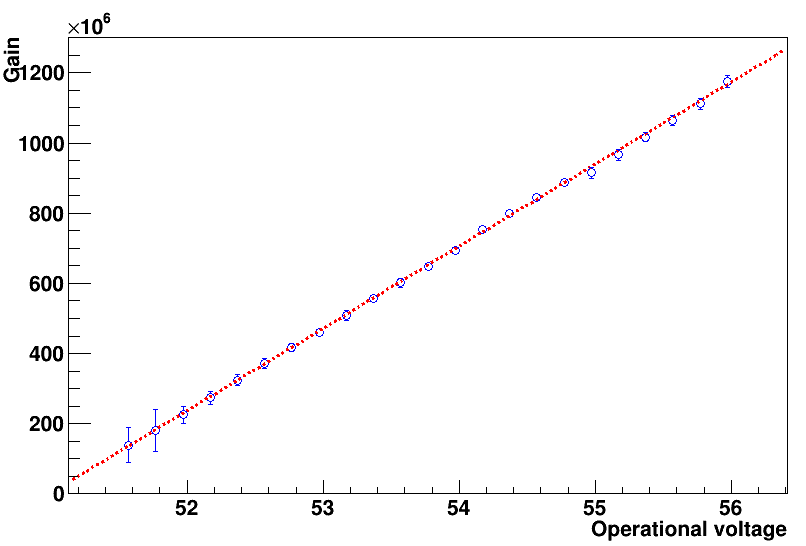
\includegraphics[scale=0.4]{Dependenciavoltaje.png}
\caption{\textbf{Figura 12}.- Ganancia frente a voltaje operacional}
\end{figure}

Podemos apreciar de nuevo la existencia de un comportamiento lineal casi perfecto en un rango de voltaje de 5 voltios. Vemos de nuevo reflejada la propiedad de buena linealidad que caracteriza a los SiPM. En la gráfica podemos notar la existencia de un mayor error en las medidas de voltajes mas bajos (en valor absoluto). Esto es debido a que nos estamos acercando al voltaje break down donde el silicio entra en modo Geiger y el valor de la ganancia empieza a ser distinto de cero. Podemos hachacar este mayor error a que a estos voltajes cercanos a la frontera de cambio de comportamiento, el SiPM todavía no funciona de forma adecuada debido a efectos más sutiles. Este necesita estar totalmente dento del modo Geiger para funcionar perfectamente. Hay que tener en cuenta además que solo se llego hasta el voltaje $V_{op}=51,57$ V debido a que, cuando estamos a valores muy cercanos al voltaje de break down la ganancia sufre un decaimiento exponencial, siendo imposible realizar su medida.

De nuevo comprobamos la calidad del ajuste a partir del test $\chi^2$ obteniendo un valor de $\frac{\chi^2}{ndf}=\frac{7.963}{21}\approx 0.379$, el cual se trata de un valor relativamente bueno.

Podemos observar que, al contrario de lo que ocurría con la temperatura, el valor de la ganancia del SiPM aumenta a medida que aumenta el voltaje operacional. Esto es debido a que a medida que aumentamos el voltaje operacional aumenta la diferencía de potencial en la zona de desertización. De esta forma, por un lado, aumentando la zona de desertización, por lo que los pares electrón--hueco dispondrán de mayor espacio para generar una mayor replicación y, por otro lado, estamos aplicando una mayor tensión sobre los pares electrón-hueco generados al detectar radiación y, por extensión, estos se verán acelerádos más rápidamente. Debido a ello dispondrán de una mayor energía para producir un mayor número de pares electrón-hueco. En resumen ambos procesos contribuyen a aumentar la ganancia del SiPM.

La ecuación obtenida en este ajuste $G=cV_{op}+d$ toma los siguientes valores: 
$$c=2.34123 \cdot 10^8 \pm 2.55246 \cdot 10^6~V^{-1}$$
$$d=-1.19368 \cdot 10^{10} \pm 1.38112 \cdot 10^8~V^{-1}$$

Remarquemos de nuevo la importancia de este resultado, no por el resultado numérico, sino porque es la parte que nos faltaba para poder calcular la compensación de la ganancia.

A demás, a modo de comprobación, podemos obtener el Voltage break down a partir de esta expresión, que se corresponde al voltaje al cual la ganancia es cero (voltage a partir del cual estamos en modo geiger y la ganancia empieza a ser no nula). El voltage calculado es: 
$$G=0=c \cdot V_{BD} +d \longrightarrow V_{BD}=-\frac{d}{c}=50.9852~V$$

Vemos que este se acerca de forma extraordinaria al voltaje teórico especificado por hamamatsu, $50.97~V$.
\end{itemize}